\documentclass[a4paper,12pt]{article}

\usepackage[utf8]{inputenc}
\usepackage[T1]{fontenc}
\usepackage[pdftex]{graphicx}
\usepackage[english, russian]{babel} % Языки: русский, английский
\usepackage[pdftex]{graphicx}
\usepackage{textcase}
\usepackage{amssymb,amsmath,amsthm,amsfonts}
\usepackage{geometry}
\geometry{a4paper,top=2cm,bottom=2cm,left=3cm,right=1cm}

\theoremstyle{plain}

\newtheorem{definition}{Определение}[section]
\newtheorem{lemma}{Лемма}[section]
%\newtheorem{proof}{Доказательство}
\newtheorem{theorem}{Теорема}[section]
%\numberwithin{equation}[section]

\begin{document}


\thispagestyle{empty}


\begin{center}
	\MakeTextUppercase{Белорусский Государственный Университет}\par 
	\MakeTextUppercase{Факультет Прикладной Математики и Информатики}\par
	Кафедра математического моделирования и анализа данных
	\par
\end{center}

\vspace*{3cm}
\begin{center}
	{\bf \large Шимко Андрея Чеславовича}
\end{center}
\vspace*{1cm}
\begin{center}
	{\bf \large Обнаружение вкраплений в двоичную цепь Маркова на основе энтропийных характеристик}
\end{center}

\vspace*{1cm}

\begin{center}
	Отчет по преддипломной практике
\end{center}
\begin{center}
	студента 5 курса 9 группы
\end{center}


\vspace{5cm}

\begin{flushright}
	\begin{tabular}{l}
		Научный руководитель:\\
		старший преподаватель\\
		Егор Валентинович Вечерко
	\end{tabular}
\end{flushright}


\par\vspace*{\fill}

\begin{center}
	{Минск, 2017}
\end{center}
\newpage


\thispagestyle{empty}

 
\clearpage

\newpage
\section{Введение}
\vspace*{1cm}

Стеганография представляет собой специфическую область человеческой деятельности, связанной с
разработкой и анализом методов сокрытия факта передачи информации. Подобно криптографии,
стеганография известна со времен античности. Но на этом аналогии, по крайне мере в контексте
теоретических исследований, заканчиваются. За последние четверть века возникла и успешно раз-
вивается новая математическая дисциплина криптология, или, что то же самое, математическая
криптография, изучающая математические модели криптографических схем. Попытки создания ма-
тематической стеганографии (которую, быть может, следует именовать также стеганологией) пред-
принимаются, но исследования здесь находятся лишь в зачаточном состоянии.\\
Такое положение дел обусловлено прежде всего сложностью возникающих в стеганографии задач. Всякая попытка построения математических моделей стеганографических систем сопряжена с
необходимостью рассмотрения большого количества случаев и подслучаев, не допускающих простой
и единообразной трактовки. Другими словами, внешняя среда, в которой должны функционировать
стеганографические системы, имеет гораздо большее, по сравнению с внешней средой криптографических схем, количество степеней свободы.\\
Основными критериями для оценки и сравнения различных методов построения стеганографических систем являются их стойкость и емкость. В отличие от достаточно исследованных криптографических систем, оценки стойкости стегосистем более сложны и само понятие стойкости имеет большое число различных формулировок, что объясняется разнообразием задач стеганографи-ческой защиты данных. В настоящей работе исследуются методы построения стегосистем, предназначенных для скрытия факта передачи конфиденциальных сообщений. Говоря о стойкости криптографических систем, важно упомянуть о принципе Керкхоффса, который заключается в том, что система защиты информации должна обеспечивать свои функции даже при полной информированности противника о ее структуре и алгоритмах, и вся секретность системы должна заключаться в ключе. Этот принцип также можно соотнести с определением стойкости стегосистем. В данном случае, ключом может являться, например, секретная последовательность, определяющая порядок прохода, элементов контейнера при внедрении бит информации, что имеет место в алгоритмах рассеянного заполнения контейнеров. Второй критерий, емкость метода, определяет максимальное количество встраиваемой информации, и может выражаться в единицах бит на пиксель.


\newpage
\section{Основные понятия}
\vspace*{1cm}
\begin{definition}\label{stegonagraphy}
Стеганография - наука о способах передачи (хранения) скрытой информации, при которых скрытый канал организуется на базе и внутри открытого канала с использованием особенностей восприятия информации, причем для этой цели могут использоваться такие приемы, \cite{agranovskiy}как:
\begin{enumerate}
	\item Полное сокрытие факта существования  скрытого канала связи
	\item Создание трудностй для обнаружения, извлечения и модификации передаваемых скрытых сообщений внутри открытых сообщений-контейнеров
	\item Маскировки скрытой информации в протоколе
\end{enumerate}
\end{definition}

\begin{definition}\label{container}
	Контейнером $b \in B$ (носителем) называют несекретные данные, которые используют для сокрытия сообщения \cite{agranovskiy}.
\end{definition}

\begin{definition}\label{message}
	Сообщение $m \in M$ - секретная информация, наличие которой в контейнере необходимо скрыть \cite{agranovskiy}.
\end{definition}

\begin{definition}\label{key}
	Ключ $k \in K$ - секретная информация, известная только законному пользователю, которая определяет конкретный вид алгоритма сокрытия \cite{agranovskiy}.
\end{definition}

\begin{definition}\label{free container}
	Пустой контейнер - контейнер, не содержащий сообщения \cite{agranovskiy}.
\end{definition}

\begin{definition}\label{full container}
	Заполненный контейнер - контейнер, с внедренным в него сообщением \cite{agranovskiy}.
\end{definition}

\begin{definition}\label{algoritm}
	Стеганографический алгоритм - два преобразования: прямое стеганографическое преобразование $F:M \times B \times K \to B$ и обратное стеганографическое преобразование $F^{-1}:B \times K \to M$, сопоставляющее соответственно тройке (сообщение, пустой контейнер, ключ) контейнер-результат и паре (заполненный контейнер, ключ) - исходное сообщение, \cite{agranovskiy}причем:
	\begin{equation}\label{algoritm equation}
		F(m, b, k) = b_{m,k}, F^{-1}(b_{m,k}, k) = m, m \in M, b_{m,k}, b \in B, k \in K
	\end{equation}
\end{definition}

\begin{definition}\label{stenography system}
	Под стеганографической системой будем понимать $S=(F, F^{-1}, M, B, K)$, представляющую собой совокупность сообщений, секретных ключей, контейнеров и связывающих их преобразований \cite{agranovskiy}.
\end{definition}

\begin{definition}\label{input}
	Внедрение (сокрытие) - применение прямого стегонаграфического преобразования к конкретным контейнеру, ключу и сообщению \cite{agranovskiy}.
\end{definition}

\begin{definition}\label{inside}
	Извлечение сообщения - применение обатного стегонаграфического преобразованияю \cite{agranovskiy}.
\end{definition}

\begin{definition}\label{l-gramm}
	l-грамм - подпоследовательность из l подряд иущих элементов последовательности.
\end{definition}

\begin{definition}
	Под дискретным источником сообщений будем понимать устройство, порождающее последовательности, составленные из букв конечного алфавита А (|A|=n<$\infty$). При этом буквы последовательностей пораждаются в дискретный момент времени:$ t = 0, 1, 2, ...; t = ...,-2, -1, 0, 1, 2, ...;$ \cite{duhin}
\end{definition}
\begin{definition}
	Если вероятность того, что источник порождает некоторую поседовательность $a_{i_1}...a_{i_l}$, составленную из букв алфавита А, в момент времени 1, 2, ... l, равна вероятности того, что порождается точно такая же последовательность в момент времени j+1, ..., j+l для любых j,l;$a_{j_1}...a_{j_l}$, то источник называется стационарным.\cite{duhin}
	Стационарность означает неизменность во времени всех конечномерных распределений соответствующего случайного процесса.
\end{definition}
\begin{definition}
	Энтропией источника назовем величину: 
	\begin{equation}
	H_\infty = \lim_{l \to \infty} \frac{H(C_l)}{l};
	 \end{equation}
	 если данный предел существует\cite{duhin}.
\end{definition}
 \clearpage

\newpage

\section{Теоретико-информационный подход к оценке стойкости систем}
\vspace*{1cm}
В настоящем разделе рассматривается теоретико-информационный подход к определению стойкости
стеганосистем для стеганографических каналов без повторений в присутствии пассивного противника,
обладающего неограниченными вычислительными возможностями.\\
В основе всех известных определений стойкости стеганосистем лежит требование неотличимости
распределения вероятностей на множестве стего от распределения вероятностей на множестве пустых
контейнеров. Рассматривается статистическая неотличимость, или, иначе говоря,
неотличимость относительно произвольных алгоритмов. \\
Парадигма неотличимости распределений вероятностей заимствована из математической криптографии. Заметим, однако, что ее адекватность для стеганографии не очевидна. По крайней мере, в
случае стеганографического канала без повторений не ясно, насколько оправданными будут усилия
отправителя по имитации распределения вероятностей на множестве пустых контейнеров. Не следует
ли вместо этого стремиться передать скрытое сообщение в одном из наиболее вероятных контейнеров?\\
Вполне очевидна идея создания стеганографического канала путем
маскировки скрытого сообщения под шум, вносимый алгоритмом шифрования в исходный контейнер. \\
Проверка гипотезы о стойкости системы состоит в том, чтобы определить, какая из двух гипотез - $H_0$ или $H_1$ - является верным толкованием наблюдаемой величины Q. Есть два возможных распределения вероятностей, которые принято обозначать $P_{Q_0}, P_{Q_1}$, над пространством возможных наблюдений. Если верна гипотеза $H_0$, тогда Q была пораждена согласно $P_{Q_0}$, если же верна гипотеза $H_1$, тогда Q  была пораждена согласно $P_{Q_1}$. Правило принятия решения - это двоичное отображение, заданное на пространстве возможных наблюдений, которое составляет одну из двух возможных гипотез для каждого возможного элемента q.
Основной мерой проверки гипотезы является относительная энтропия или различие между двумя распределениями вероятности $P_{Q_0}$ и $P_{Q_1}$, определяемое следующим выражением:
	\begin{equation}
		H(P_{Q_0}||P_{Q_1}) = \sum_{q}P_{Q_0}(q)log\frac{P_{Q_0}(q)}{P_{Q_1}(q)};
	\end{equation}
Относительная энтропия между двумя распределениями всегда неотрицательна и равна нулю только тогда, когда распределения равномерны. Несмотря на то, что отностиельная энтропия не является метрикой с точки зрения математики (так как не симметрична и не удовлетворяет аксиоме треугольника), полезно считать ее таковой. Двоичная относительная энтропия $d(\alpha, \beta)$ определяется как:
	\begin{equation}
	d(\alpha, \beta) = \alpha \log \frac{\alpha}{1-\beta} + (1-\alpha)\log \frac{1-\alpha}{\beta};
	\end{equation}
где $\alpha$  - вероятность ошибки первого рода, $\beta$  - вероятность ошибки второго рода.

\newpage
\section{Математическая модель вкраплений на основе схемы независимых испытаний}

\vspace*{1cm}
Контейнер представляет собой последовательность случайных величин распределенных по закону Бернулли с параметром p:
\begin{equation}\label{container:eq}\
	\mathcal{L}{x_t} = Bi(1, p), x_i \in V = {0, 1}, i = \overline{1,T};
\end{equation}
Вкрапляемое сообщение имеет вид:
\begin{equation}
	\mathcal{L}{m_t} = Bi(1, \theta), m_i \in V = {0, 1}, i = \overline{1,\tau};
\end{equation}
Ключ $\gamma_t$ определяет момент времени вкрапления i-того бита сообщения в исходный контейнер:
\begin{equation}
	\mathcal{L}{\gamma_t} = Bi(1, \delta), \gamma_i \in V = {0, 1}, i = \overline{1,T};
\end{equation}
Вкрапление битов ${m_t}$ производится по правилу, заданному следующим функциональным преобразованием:
\begin{equation}\label{input:rule}
	y_t=(1-\gamma_t)x_t+\gamma_t m_{\tau_t};
\end{equation}

\begin{lemma}\label{lemma:1}
	Для модели (\ref{container:eq})-(\ref{input:rule})
	\begin{equation}
		P\{y_t=1\}=(1-\delta)p+\delta\theta;
	\end{equation}
	\begin{equation}
		P\{y_t=0\} = (1-\delta)(1-p)+ \delta(1-\theta);
	\end{equation}
\end{lemma}
\begin{proof}
	Воспользуемся формулой полной вероятности:\\
	$P\{y_t=1\}=P\{(1-\gamma_t)x_t + \gamma_t m_{\tau_t} =1\} = \sum_{j \in V} P\{y_t = 1, \gamma_t = j\} =\sum_{j \in V} P\{\gamma_t = j\} P\{y_t = 1|\gamma_t = j\} = (1-\delta)P\{x_=1, \gamma_t=0\} + \delta P\{m_{\tau_t}=1, \gamma_t =1\} = (1-\delta)p + \delta\theta;\\$
	Тогда:\\
	$P\{y_t = 0\} = 1 - P\{y_t = 1\}= (1-\delta)(1-p)+\delta(1-\theta);$
\end{proof} 
\begin{equation}
	h = \frac{H(y_1,...,y_t)}{T} = \frac{TH(y_1)}{T}=H(y_1);
\end{equation}
Воспользуемся леммой \ref{lemma:1}:\newline
$
h = -P\{y_t=1\}\log_2 P(y_t = 1)-P\{y_t=0\}\log_2 P(y_t = 0) = - ((1-\delta)p+\delta\theta)\log_2 ((1-\delta)p+\delta\theta) - ((1-\delta)(1-p) + \delta(1-\theta))\log_2((1-\delta)(1-p) + \delta(1-\theta)).
$



\newpage
\section{Математическая модель вкраплений в двоичную стационарную марковскую последовательность 1-го порядка и ее свойства}

Рассмотрим модель (\ref{container:eq})-(\ref{input:rule}).

Пусть контейнер (\ref{container:eq}) пердставляет собой цепь Маркова 1-го порядка с вектором распределения вероятностей $\pi = (\frac{1}{2}, \frac{1}{2})$ и матрицей вероятностей одношаговых переходов
\begin{equation}\label{markov:rule} 
	P(\varepsilon)=\frac{1}{2}\bigl( \begin{matrix}
		1+\varepsilon,  1-\varepsilon\\
		1-\varepsilon,  1+\varepsilon
	\end{matrix}\bigl), |\varepsilon|<1, \varepsilon \neq 0.
\end{equation}
\begin{lemma}
	Для модели (\ref{container:eq})-(\ref{input:rule}) с условием (\ref{markov:rule}):
	\begin{equation}\label{1:1}
		P\{y_{t-1}=1, y_t = 1 \}=\frac{1}{4}(1+\varepsilon)(1-\delta)^2+\theta\delta(1-\delta)+\theta^2\delta^2;
	\end{equation}
	\begin{equation}\label{0:1}
		P\{y_{t-1}=1, y_t = 0 \}=\frac{1}{4}(1-\varepsilon)(1-\delta)^2+\frac{1}{2}\delta(1-\delta)+\theta(1-\theta)\delta^2;
	\end{equation}
	\begin{equation}
		P\{y_{t-1}=0, y_t = 1 \}=\frac{1}{4}(1-\varepsilon)(1-\delta)^2+\frac{1}{2}\delta(1-\delta)+\theta(1-\theta)\delta^2;
	\end{equation}
	\begin{equation}\label{0:0}
		P\{y_{t-1}=0, y_t = 0 \}=\frac{1}{4}(1+\varepsilon)(1-\delta)^2+\delta(1-\theta)(1-\delta)+\delta^2(1-\theta)^2.
	\end{equation}
\end{lemma}
\begin{proof}
	Рассмотрим биграмм: $\{y_{t-1}, y_t\}$\\
	$(a_1, a_2) \in \{0,1\}, P\{y_{t-1}=a_1, y_t=a_2\} = \sum_{(b_1, b_2)\in \{0, 1\}^2} P\{y_{t-1} = b_1, y_t = b_2, \gamma_{t-1}=a_1, \gamma_t = a_2\}= \sum_{(b_1, b_2)\in \{0, 1\}^2} P\{y_{t-1} = b_1, y_t = b_2| \gamma_{t-1}=a_1, \gamma_t = a_2\}P\{\gamma_{t-1}=a_1, \gamma_t = a_2\}.$\\
	Для (\ref{1:1}):\\
	$\sum_{(b_1, b_2)\in \{0, 1\}^2} P\{y_{t-1} = b_1, y_t = b_2| \gamma_{t-1}=a_1, \gamma_t = a_2\}P\{\gamma_{t-1}=a_1, \gamma_t = a_2\}=\frac{1}{2}\cdot\frac{1}{2}(1+\varepsilon)(1-\delta)^2+\theta\delta(1-\theta) + \theta^2\delta^2.$\\
	Для случаев (\ref{0:1})-(\ref{0:0}) доказывается аналогично.	
\end{proof}
Для формул (\ref{1:1})-(\ref{0:0}) справедливо условие нормировки:\\
$ \sum_{(a_1, a_2)\in \{0, 1\}^2}P\{y_{t-1}=a_1, y_t=a_2\} =1.$\\
Далее полагаем, что $\theta=\frac{1}{2}$.\\
Тогда: 
\begin{equation}
	P\{y_{t-1}=1, y_t = 1 \}=P\{y_{t-1}=0, y_t = 0 \}= \delta^2\frac{\varepsilon}{4}-\delta\frac{\varepsilon}{2}+\frac{1+\varepsilon}{4};
\end{equation}
\begin{equation}
	P\{y_{t-1}=1, y_t = 0 \}=P\{y_{t-1}=0, y_t = 1 \}= -\delta^2\frac{\varepsilon}{4}+\delta\frac{\varepsilon}{2}+\frac{1-\varepsilon}{4}.
\end{equation}
\begin{definition}
	\cite{duhin} Дискретный стационарный источник называется марковским источником порядка m, если для любого l(l>m) и любой последовательности $c_l=(a_{i_1}, ..., a_{i_l})$ выполняется: $P\{a_{i_l}|a_{i_{l-1}}, ..., a_{i_1}\} = P\{a_{i_l}|a_{i_{l-1}}, ..., a_{i_{l-m+1}}\}.$
\end{definition}
\begin{definition}
	\cite{duhin} Величина: 
	$H^{(k)} = \sum_{\{c_k\}}P\{a_{i_1}, ..., a_{i_k}\} \log{P\{a_{i_k}|a_{i_{k-1}} ..., a_{i_1}\} }$ называется шаговой энтропией марковского источника порядка k.
\end{definition}

Введем понятие энтропии на знак для l-граммы:\\
\begin{equation}
	\label{entropy L}
	H_l(\delta) = -\frac{1}{l} \sum_{(a_1, ..., a_l)\in \{0, 1\}}P\{y_{t-l}=a_1,..., y_{t-1}=a_l\}\log{P\{y_{t-l}=a_1, ..., y_{t-1}=a_l\}}.
\end{equation}
При $\delta = 0$ стегоконтейнер $y$ совпадает с контейнером $x$, тогда:\\
\begin{equation}
	H_l(0)=-\frac{1}{l}(H\{x_1\}+(l-1)H\{x_2|x_1\});
\end{equation}
\begin{equation}
	\lim_{l \to \infty}H_l(0)= \lim_{l \to \infty}-\frac{1}{l}(H\{x_1\}+(l-1)H\{x_2|x_1\}) = H\{x_2|x_1\}.
\end{equation}

Рассмотрим случайную величину $\xi \in B=\{b_1,...,b_m\}$, заданную  на вероятностном пространстве $(\Omega,\mathcal{F},\mathcal{P} )$, $P\{\xi=b_i\}=p_i$.

\begin{definition} \cite{duhin} 
	Величина 
	\begin{equation}\label{own:information}I\{b_i\}=-\log p_i
	\end{equation}
	называется собственной информацией, содержащейся в исходе $b_i \in B$. 
\end{definition}
Велиина $I\{b_i\}$ изменяется от нуля в случае
реализации достоверного исхода до бесконечности, когда $p(b_i)=p_i\rightarrow 0$.
Величину $I\{b_i\}$ можно интерпретировать как априорную неопределённость события $\{\xi=b_i\}$.

Случайная величина $I\{\xi\}$ имеет математическое ожидание
\begin{equation}
	EI\{\xi\}=-\sum_{b_i \in B}p_i\log p_i.
\end{equation}

\begin{definition}
	Величина $EI\{\xi\}$ называется средней собственной информацией.
\end{definition}
Cредняя собственная информация равна энтропии: $EI\{\xi\}=H\{\xi\}$.

Для представления функции логарифма воспользуемся формулой Маклорена первого порядка:
\begin{equation}\label{macklaren}
	f(\delta)=f(\delta_0)+(\delta-\delta_0)f'(\delta_0)+o((\delta-\delta_0)^2).
\end{equation}

Для краткости, в обозначении функции $\log$ будем использовать основание $b$. 

Согласно (\ref{macklaren}) в точке $\delta=0$ справедливо асимптотическое разложение 1-го порядка:
\begin{gather*}
	\log_b(a_0(\varepsilon)+\delta a_1(\varepsilon) + \delta^2 a_2(\varepsilon) + o(\delta^2)) = \\ =
	\log a_0(\varepsilon)+\delta \left(\log(a_0(\varepsilon)+\delta a_1(\varepsilon) + \delta^2 a_2(\varepsilon) + o(\delta^2))\right)'|_{\delta=0} + o(\delta)= \\=
	\log a_0(\varepsilon) +\delta \frac{1}{\ln b}\frac{a_1(\varepsilon)}{a_0(\varepsilon)}+o(\delta).
\end{gather*}

Учитывая (\ref{macklaren}), найдем асимптотические выражения при $\delta \rightarrow 0$ для собственной информации $I\{y_{t-1}=i_1, y_t = i_2 \}, i_1,i_2 \in \{0,1\}$:
\begin{gather*}
	I\{y_{t-1}=0, y_t = 0 \}=I\{y_{t-1}=1, y_t = 1 \}= -\log(\frac{1}{4}(1+\varepsilon)(1-\delta)^2+\frac{1}{2}\delta(1-\delta)+\frac{1}{4}\delta^2) =\\=
	-\log \frac{1+\varepsilon}{4} + \delta \frac{1}{\ln b}\frac{2\varepsilon}{1+\varepsilon} + o(\delta);
	\\
	I\{y_{t-1}=0, y_t = 1 \}=I\{y_{t-1}=1, y_t = 0 \}= -\log(\frac{1}{4}(1-\varepsilon)(1-\delta)^2+\frac{1}{2}\delta(1-\delta)+\frac{1}{4})\delta^2) =\\= 
	-\log \frac{1-\varepsilon}{4} - \delta \frac{1}{\ln b}\frac{2\varepsilon}{1-\varepsilon} + o(\delta).
\end{gather*}

\begin{lemma}
	Если имеет место монобитная модель вкраплений (\ref{container:eq})-(\ref{input:rule}), то для энтропии при $l=2$ справедливо асимптотическое разложение 1-го порядка
	\begin{equation}
		H_2(\delta) = H_2(0) + 2\delta\varepsilon\log\frac{1+\varepsilon}{1-\varepsilon}+O(\delta^2).
	\end{equation}
\end{lemma}
\begin{proof}
	$H_2(\delta)= -( P\{y_{t-1}=0, y_t = 0\}\log(P\{y_{t-1}=0, y_t = 0\}) + P\{y_{t-1}=0, y_t = 1\}\log(P\{y_{t-1}=0, y_t = 1\}) +P\{y_{t-1}=1, y_t = 0\}\log(P\{y_{t-1}=1, y_t = 0\}) +P\{y_{t-1}=1, y_t = 1\}\log(P\{y_{t-1}=1, y_t = 1\})) = -2 (P\{y_{t-1}=0, y_t = 0\}\log(P\{y_{t-1}=0, y_t = 0\}) +P\{y_{t-1}=0, y_t = 0\}\log(P\{y_{t-1}=0, y_t = 1\}) )=-2((\delta^2\frac{\varepsilon}{4}-\delta\frac{\varepsilon}{2}+\frac{1+\varepsilon}{4})(-\log(\frac{1+\varepsilon}{4})+ \delta \frac{1}{\ln b}\cdot \frac{2\varepsilon}{1+\varepsilon}+o(\delta^2)) + (-\delta^2\frac{\varepsilon}{4}+\delta\frac{\varepsilon}{2}+\frac{1-\varepsilon}{4})(-\log(\frac{1-\varepsilon}{4}) - \delta \frac{1}{\ln b}\cdot \frac{2\varepsilon}{1-\varepsilon}+o(\delta^2)))=\frac{1}{2}(-(1+\varepsilon) \log(\frac{1+\varepsilon}{4}) - (1-\varepsilon)\log(\frac{1-\varepsilon}{4}) + 2\delta\varepsilon\log(\frac{1+\varepsilon}{1-\varepsilon})))+O(\delta^2) =H_2(0) + 2\delta\varepsilon\log(\frac{1+\varepsilon}{1-\varepsilon})))+O(\delta^2).$
\end{proof}

\begin{definition}\cite{duhin}
	Величина $\lim_{k\to \infty}H^{(k)}= \lim_{k\to \infty}H_{k}=H_{\infty} \geqslant 0$  называется энтропий марковского источника, где $H_{k}$ - энтропия на знак.
\end{definition}

Рассмотрим  условные вероятности появления трехграммы $(0,0,0)$ при условии всевозможных стегоключей.

$P\{y_{i-1} = 0, y_i = 0, y_{i+1} = 0\} =  (1-\delta)^3P\{y_{i-1} = 0, y_i = 0, y_{i+1} = 0 |\gamma_{i-1}=0,\gamma_i=0,\gamma_{i+1}=0\} +\newline + 
\delta(1-\delta)^2 (P\{y_{i-1} = 0, y_i = 0, y_{i+1} = 0 |\gamma_{i-1}=1,\gamma_i=0,\gamma_{i+1}=0\} + P\{y_{i-1} = 0, y_i = 0, y_{i+1} = 0 |\gamma_{i-1}=0,\gamma_i=1,\gamma_{i+1}=0\} + P\{y_{i-1} = 0, y_i = 0, y_{i+1} = 0 |\gamma_{i-1}=0,\gamma_i=0,\gamma_{i+1}=1\})+\newline 
+\delta^2(1-\delta) (P\{y_{i-1} = 0, y_i = 0, y_{i+1} = 0 |\gamma_{i-1}=1,\gamma_i=1,\gamma_{i+1}=0\}  + P\{y_{i-1} = 0, y_i = 0, y_{i+1} = 0 |\gamma_{i-1}=0,\gamma_i=1,\gamma_{i+1}=1\} + P\{y_{i-1} = 0, y_i = 0, y_{i+1} = 0 |\gamma_{i-1}=1,\gamma_i=0,\gamma_{i+1}=1\}) + \newline 
+ \delta^3 (P\{y_{i-1} = 0, y_i = 0, y_{i+1} =0 | \gamma_{i-1}=1,\gamma_i=1,\gamma_{i+1}=1\}).$\newline



$P\{y_{i-1} = 0, y_i = 0, y_{i+1} = 0|\gamma_1=0,\gamma_2=0,\gamma_3=0\} = P\{x_{i-1} = 0, x_i = 0, x_{i+1} = 0\} = P\{x_{i-1} = 0\}P\{x_i=0, x_{i+1}=0 | x_{i-1} = 0\} = P\{x_{i-1} = 0\}P\{x_i=0\}P\{ x_{i+1}=0 | x_{i} = 0\}  = \frac{1}{2}\cdot\frac{1}{2}(1+\varepsilon)\cdot\frac{1}{2}(1+\varepsilon)=\frac{1}{8}(1+\varepsilon)^2;$\newline

$P\{y_{i-1} = 0, y_i = 0, y_{i+1} = 0|\gamma_1=1,\gamma_2=0,\gamma_3=0\} = P\{\xi = 0, x_i = 0, x_{i+1} = 0\} = P\{\xi = 0\}P\{x_i=0, x_{i+1}=0 \} = P\{\xi = 0\}P\{x_i=0\}P\{ x_{i+1}=0 | x_{i} = 0\}  = \frac{1}{2}\cdot\frac{1}{2}(1+\varepsilon)\cdot\frac{1}{2}=\frac{1}{8}(1+\varepsilon);$\newline 

$P\{y_{i-1} = 0, y_i = 0, y_{i+1} = 0|\gamma_1=0,\gamma_2=1,\gamma_3=0\} = P\{x_{i-1} = 0, \xi = 0, x_{i+1} = 0\} = P\{\xi = 0\}P\{x_{i-1}=0, x_{i+1}=0 \}  = \frac{1}{2}\cdot\frac{1}{2}\cdot\frac{1}{2}(1+\varepsilon^2)=\frac{1}{8}(1+\varepsilon^2);$\newline


$P\{y_{i-1} = 0, y_i = 0, y_{i+1} = 0|\gamma_1=0,\gamma_2=0,\gamma_3=1\} = P\{x_{i-1} = 0, x_i = 0, \xi = 0\} = P\{\xi = 0\}P\{x_{i-1}=0, x_{i}=0 \}  = \frac{1}{2}\cdot\frac{1}{2}\cdot\frac{1}{2}(1+\varepsilon)=\frac{1}{8}(1+\varepsilon);$\newline

$P\{y_{i-1} = 0, y_i = 0, y_{i+1} = 0|\gamma_1=0,\gamma_2=1,\gamma_3=1\} = P\{y_{i-1} = 0, y_i = 0, y_{i+1} = 0|\gamma_1=1,\gamma_2=0,\gamma_3=1\} =
P\{y_{i-1} = 0, y_i = 0, y_{i+1} = 0|\gamma_1=1,\gamma_2=1,\gamma_3=0\} =
P\{y_{i-1} = 0, y_i = 0, y_{i+1} = 0|\gamma_1=1,\gamma_2=1,\gamma_3=1\} = P\{\xi = 0, \xi = 0, \xi = 0\} = P\{\xi = 1\}P\{x_{i-1}=1\}P\{x_{i}=0 \}  = \frac{1}{2}\cdot\frac{1}{2}\cdot\frac{1}{2} = \frac{1}{8};$\newline

$P\{y_{i-1} = 0, y_i = 0, y_{i+1} = 0\} =  \frac{1}{8}\bigr(\varepsilon(\varepsilon+2)\delta^2 - 2\varepsilon(\varepsilon+1)\delta + (1+\varepsilon)^2 \bigr).$\newline

Найдем вероятности появления всевозможных трехграмм в стегоконтейнере $\{y_t\}$:
\begin{gather*}
	P\{y_{i-1} = 1, y_i = 1, y_{i+1} = 1\} = P\{y_{i-1} = 0, y_i = 0, y_{i+1} = 0\}=\\=\tfrac{1}{8}\bigr(\varepsilon(\varepsilon+2)\delta^2 - 2\varepsilon(\varepsilon+2)\delta + (1+\varepsilon)^2 \bigr),\\
	P\{y_{i-1} = 1, y_i = 1, y_{i+1} = 0\} = P\{y_{i-1} = 0, y_i = 0, y_{i+1} = 1\}= P\{y_{i-1} = 0, y_i = 1, y_{i+1} = 1\} =\\= P\{y_{i-1} = 1, y_i = 0, y_{i+1} = 0\}   =\tfrac{1}{8}\bigr(-\varepsilon^2\delta^2 + 2\varepsilon^2\delta  -\varepsilon^2 + 1\bigr), \\
	P\{y_{i-1} = 1, y_i = 0, y_{i+1} = 1\} = P\{y_{i-1} = 0, y_i = 1, y_{i+1} = 0\}=\\=\tfrac{1}{8}\bigr(\varepsilon(\varepsilon-2)\delta^2 - 2\varepsilon(\varepsilon-2)\delta + (1-\varepsilon)^2 \bigr).
\end{gather*}

\begin{theorem}
	Если имеет место монобитная модель вкраплений (\ref{container:eq})-(\ref{input:rule}) , то для энтропии при $l=3$ справедливо асимптотическое разложение 1-го порядка:
	\begin{equation}
		H_3(\delta)=H_3(0)+2\varepsilon\delta \log\frac{1+\varepsilon}{1-\varepsilon}+ O(\delta^2);
	\end{equation}
	собственная информация имеет вид:
	\begin{gather*}
		I\{y_{i-1} = 0, y_i = 0, y_{i+1} = 0\}=-\log\frac{(1+\varepsilon)^2}{8}+\delta\frac{1}{\ln b}\cdot\frac{2\varepsilon^2+4\varepsilon}{(1+\varepsilon)^2} + O(\delta^2), \\
		I\{y_{i-1} = 1, y_i = 0, y_{i+1} = 0\}= I\{y_{i-1} = 0, y_i = 0, y_{i+1} = 1\}=\\=
		-\log\frac{1-\varepsilon^2}{8}-\delta\frac{1}{\ln b}\cdot\frac{2\varepsilon^2}{1-\varepsilon^2} + O(\delta^2),\\
		I\{y_{i-1} = 0, y_i = 1, y_{i+1} = 0\}= -\log\frac{(1-\varepsilon)^2}{8}+\delta\frac{1}{\ln b}\cdot\frac{2\varepsilon^2-4\varepsilon}{(1-\varepsilon)^2} + O(\delta^2);\\
		I\{y_{i-1} = j_{1}, y_i = j_2, y_{i+1} = j_{3}\}=I\{y_{i-1} = 1-j_{1}, y_i = 1-j_2, y_{i+1} = 1-j_{3}\}, ~j_1,j_2,j_3 \in \{0,1\}.
	\end{gather*}		
\end{theorem}
\begin{proof}
	Подставляя в (\ref{macklaren}) найденные выражения для вероятностей трехграмм, получим асимптотические выражения для собственной информации.
	
	Используя выражения для собственной информации, получим:\\
	$H_3(\delta)=-2(\frac{1}{8}\bigr(\varepsilon(\varepsilon+2)\delta^2 - 2\varepsilon(\varepsilon+2)\delta + (1+\varepsilon)^2 \bigr)( \log(\frac{(1+\varepsilon)^2}{8})+\delta\frac{1}{\ln b}\cdot\frac{-2\varepsilon^2-4\varepsilon}{(1+\varepsilon)^2}) + 2\frac{1}{8}\bigr(-\varepsilon^2\delta^2 + 2\varepsilon^2\delta  -\varepsilon^2 + 1\bigr)(\log(\frac{1-\varepsilon^2}{8})+\delta\frac{1}{\ln b}\cdot\frac{2\varepsilon^2}{1-\varepsilon^2}) + \frac{1}{8}\bigr(\varepsilon(\varepsilon-2)\delta^2 - 2\varepsilon(2+\varepsilon)\delta + (1-\varepsilon)^2 \bigr)(\log(\frac{(1-\varepsilon)^2}{8})+\delta\frac{1}{\ln b}\cdot\frac{-2\varepsilon^2+4\varepsilon}{(1-\varepsilon)^2})) + O(\delta^2) =-((1-\varepsilon)\log(1-\varepsilon) + (1+\varepsilon)\log(1+\varepsilon)+\log(\frac{1}{8}) + 2\varepsilon\delta \log\frac{1-\varepsilon}{1+\varepsilon})+ O(\delta^2)=H_3(0)- 2\varepsilon\delta \log\frac{1-\varepsilon}{1+\varepsilon}+ O(\delta^2).$
\end{proof}

Рассмотрим  условные вероятности появления четырехграммы $(0,0,0,0)$ при условии всевозможных стегоключей.

$P\{y_{i-1} = 0, y_i = 0, y_{i+1} = 0, y_{i+2} = 0\} =  (1-\delta)^4P\{y_{i-1} = 0, y_i = 0, y_{i+1} = 0, y_{i+2} = 0 |\gamma_{i-1}=0,\gamma_i=0,\gamma_{i+1}=0, \gamma_{i+2} = 0\} + 
\delta(1-\delta)^3\biggr(P\{y_{i-1} = 0, y_i = 0, y_{i+1} = 0, y_{i+2} = 0 |\gamma_{i-1}=0,\gamma_i=0,\gamma_{i+1}=0, \gamma_{i+2} = 1\} +
P\{y_{i-1} = 0, y_i = 0, y_{i+1} = 0, y_{i+2} = 0 |\gamma_{i-1}=0,\gamma_i=0,\gamma_{i+1}=1, \gamma_{i+2} = 0\} +
P\{y_{i-1} = 0, y_i = 0, y_{i+1} = 0, y_{i+2} = 0 |\gamma_{i-1}=0,\gamma_i=1,\gamma_{i+1}=0, \gamma_{i+2} = 0\} +
P\{y_{i-1} = 0, y_i = 0, y_{i+1} = 0, y_{i+2} = 0 |\gamma_{i-1}=1,\gamma_i=0,\gamma_{i+1}=0, \gamma_{i+2} = 0\}\biggr) +
\delta^2(1-\delta)^2 \biggr(P\{y_{i-1} = 0, y_i = 0, y_{i+1} = 0, y_{i+2} = 0 |\gamma_{i-1}=0,\gamma_i=0,\gamma_{i+1}=1, \gamma_{i+2} = 1\} +
P\{y_{i-1} = 0, y_i = 0, y_{i+1} = 0, y_{i+2} = 0 |\gamma_{i-1}=0,\gamma_i=1,\gamma_{i+1}=1, \gamma_{i+2} = 0\} +
P\{y_{i-1} = 0, y_i = 0, y_{i+1} = 0, y_{i+2} = 0 |\gamma_{i-1}=1,\gamma_i=1,\gamma_{i+1}=0, \gamma_{i+2} = 0\} +
P\{y_{i-1} = 0, y_i = 0, y_{i+1} = 0, y_{i+2} = 0 |\gamma_{i-1}=1,\gamma_i=0,\gamma_{i+1}=1, \gamma_{i+2} = 0\}+
P\{y_{i-1} = 0, y_i = 0, y_{i+1} = 0, y_{i+2} = 0 |\gamma_{i-1}=0,\gamma_i=1,\gamma_{i+1}=0, \gamma_{i+2} = 1\}+
P\{y_{i-1} = 0, y_i = 0, y_{i+1} = 0, y_{i+2} = 0 |\gamma_{i-1}=1,\gamma_i=0,\gamma_{i+1}=0, \gamma_{i+2} = 1\}\biggr)
+\delta^3(1-\delta) \biggr(P\{y_{i-1} = 0, y_i = 0, y_{i+1} = 0, y_{i+2} = 0 |\gamma_{i-1}=0,\gamma_i=1,\gamma_{i+1}=1, \gamma_{i+2} = 1\} +
P\{y_{i-1} = 0, y_i = 0, y_{i+1} = 0, y_{i+2} = 0 |\gamma_{i-1}=1,\gamma_i=0,\gamma_{i+1}=1, \gamma_{i+2} = 1\} +
P\{y_{i-1} = 0, y_i = 0, y_{i+1} = 0, y_{i+2} = 0 |\gamma_{i-1}=1,\gamma_i=1,\gamma_{i+1}=0, \gamma_{i+2} = 1\} +
P\{y_{i-1} = 0, y_i = 0, y_{i+1} = 0, y_{i+2} = 0 |\gamma_{i-1}=1,\gamma_i=1,\gamma_{i+1}=1, \gamma_{i+2} = 0\}\biggr)
+ \delta^4 (	P\{y_{i-1} = 0, y_i = 0, y_{i+1} = 0, y_{i+2} = 0 |\gamma_{i-1}=1,\gamma_i=1,\gamma_{i+1}=1, \gamma_{i+2} = 1\}).$\newline

$P\{y_{i-1} = 0, y_i = 0, y_{i+1} = 0, y_{i+2} = 0 |\gamma_{i-1}=0,\gamma_i=0,\gamma_{i+1}=0, \gamma_{i+2} = 0\}=\frac{(1+\varepsilon)^3}{16};$\newline

$P\{y_{i-1} = 0, y_i = 0, y_{i+1} = 0, y_{i+2} = 0 |\gamma_{i-1}=1,\gamma_i=0,\gamma_{i+1}=0, \gamma_{i+2} = 0\}=P\{y_{i-1} = 0, y_i = 0, y_{i+1} = 0, y_{i+2} = 0 |\gamma_{i-1}=0,\gamma_i=0,\gamma_{i+1}=0, \gamma_{i+2} = 1\}=\frac{(1+\varepsilon)^2}{16};$\newline

$P\{y_{i-1} = 0, y_i = 0, y_{i+1} = 0, y_{i+2} = 0 |\gamma_{i-1}=0,\gamma_i=1,\gamma_{i+1}=0, \gamma_{i+2} = 0\}=P\{y_{i-1} = 0, y_i = 0, y_{i+1} = 0, y_{i+2} = 0 |\gamma_{i-1}=0,\gamma_i=0,\gamma_{i+1}=1, \gamma_{i+2} = 0\} =\frac{(1+\varepsilon)(1+\varepsilon^2)}{16};$\newline

$P\{y_{i-1} = 0, y_i = 0, y_{i+1} = 0, y_{i+2} = 0 |\gamma_{i-1}=1,\gamma_i=1,\gamma_{i+1}=0, \gamma_{i+2} = 0\}=P\{y_{i-1} = 0, y_i = 0, y_{i+1} = 0, y_{i+2} = 0 |\gamma_{i-1}=0,\gamma_i=0,\gamma_{i+1}=0, \gamma_{i+2} = 1\}=P\{y_{i-1} = 0, y_i = 0, y_{i+1} = 0, y_{i+2} = 0 |\gamma_{i-1}=1,\gamma_i=0,\gamma_{i+1}=0, \gamma_{i+2} = 1\}=P\{y_{i-1} = 0, y_i = 0, y_{i+1} = 0, y_{i+2} = 0 |\gamma_{i-1}=0,\gamma_i=0,\gamma_{i+1}=1, \gamma_{i+2} = 1\}=\frac{1+\varepsilon}{16};$\newline

$P\{y_{i-1} = 0, y_i = 0, y_{i+1} = 0, y_{i+2} = 0 |\gamma_{i-1}=0,\gamma_i=1,\gamma_{i+1}=0, \gamma_{i+2} = 1\}=P\{y_{i-1} = 0, y_i = 0, y_{i+1} = 0, y_{i+2} = 0 |\gamma_{i-1}=1,\gamma_i=0,\gamma_{i+1}=1, \gamma_{i+2} = 0\}=\frac{1+\varepsilon^2}{16};$\newline

$P\{y_{i-1} = 0, y_i = 0, y_{i+1} = 0, y_{i+2} = 0 |\gamma_{i-1}=1,\gamma_i=1,\gamma_{i+1}=1, \gamma_{i+2} = 0\}=P\{y_{i-1} = 0, y_i = 0, y_{i+1} = 0, y_{i+2} = 0 |\gamma_{i-1}=1,\gamma_i=1,\gamma_{i+1}=0, \gamma_{i+2} = 1\}=P\{y_{i-1} = 0, y_i = 0, y_{i+1} = 0, y_{i+2} = 0 |\gamma_{i-1}=1,\gamma_i=0,\gamma_{i+1}=1, \gamma_{i+2} = 1\}=P\{y_{i-1} = 0, y_i = 0, y_{i+1} = 0, y_{i+2} = 0 |\gamma_{i-1}=0,\gamma_i=1,\gamma_{i+1}=1, \gamma_{i+2} =P\{y_{i-1} = 0, y_i = 0, y_{i+1} = 0, y_{i+2} = 0 |\gamma_{i-1}=1,\gamma_i=1,\gamma_{i+1}=1, \gamma_{i+2}= 1\}=\frac{1}{16};$\newline

$P\{y_{i-1} = 0, y_i = 0, y_{i+1} = 0, y_{i+2} = 0 \}=P\{y_{i-1} = 1, y_i = 1, y_{i+1} = 1, y_{i+2} = 1 \}= \tfrac{1}{16}\bigr(\delta^4\varepsilon^2+\delta^3(-4\varepsilon^2)+\delta^2(\varepsilon^3+8\varepsilon^2+3\varepsilon)+\delta(-2\varepsilon^3-8\varepsilon^2-6\varepsilon)+\varepsilon^3+3\varepsilon^2+3\varepsilon+1\bigr).$\\
Найдем вероятности появления всевозможных четырехграмм в стегоконтейнере $\{y_t\}$:
\begin{gather*}
	P\{y_{i-1} = 0, y_i = 0, y_{i+1} = 0, y_{i+2} = 1 \}=P\{y_{i-1} = 1, y_i = 1, y_{i+1} = 1, y_{i+2} = 0 \}=\\=
	P\{y_{i-1} = 1, y_i = 0, y_{i+1} = 0, y_{i+2} = 0 \}=P\{y_{i-1} = 0, y_i = 1, y_{i+1} = 1, y_{i+2} = 1 \}=\\= \tfrac{1}{16}\bigr(\delta^4(-\varepsilon^2)+\delta^3\cdot4\varepsilon^2+\delta^2(-\varepsilon^3-6\varepsilon^2+\varepsilon)+\delta(2\varepsilon^3+4\varepsilon^2-2\varepsilon)-\varepsilon^3-\varepsilon^2+\varepsilon+1\bigr);\\
	P\{y_{i-1} = 0, y_i = 1, y_{i+1} = 0, y_{i+2} = 0 \}=P\{y_{i-1} = 1, y_i = 0, y_{i+1} = 1, y_{i+2} = 1 \}=\\=
	P\{y_{i-1} = 0, y_i = 0, y_{i+1} = 1, y_{i+2} = 0 \}=P\{y_{i-1} = 1, y_i = 1, y_{i+1} = 0, y_{i+2} = 1 \}=\\= \tfrac{1}{16}\bigr(\delta^4(-\varepsilon^2)+\delta^3\cdot4\varepsilon^2+\delta^2(\varepsilon^3-6\varepsilon^2-\varepsilon)+\delta(-2\varepsilon^3+4\varepsilon^2+2\varepsilon)+\varepsilon^3-\varepsilon^2-\varepsilon+1\bigr);\\
	P\{y_{i-1} = 0, y_i = 0, y_{i+1} = 1, y_{i+2} = 1 \}=P\{y_{i-1} = 1, y_i = 1, y_{i+1} = 0, y_{i+2}=0 \}=\\= \tfrac{1}{16}\bigr(\delta^4\varepsilon^2+\delta^3(-4\varepsilon^2)+\delta^2(-\varepsilon^3+4\varepsilon^2+\varepsilon)+\delta(2\varepsilon^3-2\varepsilon)-\varepsilon^3-\varepsilon^2+\varepsilon+1\bigr);\\
	P\{y_{i-1} = 0, y_i = 1, y_{i+1} = 1, y_{i+2} = 0 \}=P\{y_{i-1} = 1, y_i = 0, y_{i+1} = 0, y_{i+2} = 1 \}=\\= \tfrac{1}{16}\bigr(\delta^4\varepsilon^2+\delta^3(-4\varepsilon^2)+\delta^2(\varepsilon^3+4\varepsilon^2-\varepsilon)+\delta(-2\varepsilon^3+2\varepsilon)+\varepsilon^3-\varepsilon^2-\varepsilon+1\bigr);\\
	P\{y_{i-1} = 1, y_i = 0, y_{i+1} = 1, y_{i+2} = 0 \}=P\{y_{i-1} = 0, y_i = 1, y_{i+1} = 0, y_{i+2} = 1 \}=\\= \tfrac{1}{16}\bigr(\delta^4\varepsilon^2+\delta^3(-4\varepsilon^2)+\delta^2(-\varepsilon^3+8\varepsilon^2-3\varepsilon)+\delta(2\varepsilon^3-8\varepsilon^2+6\varepsilon)-\varepsilon^3+3\varepsilon^2-3\varepsilon+1\bigr).
\end{gather*}
\begin{theorem}
	Если имеет место монобитная модель вкраплений (\ref{container:eq})-(\ref{input:rule}) , то для энтропии при $l=4$ справедливо асимптотическое разложение 1-го порядка:
	\begin{equation}
		H_4(\delta)=H_4(0)+\frac{24\varepsilon\delta}{16} \log\frac{1+\varepsilon}{1-\varepsilon}+ O(\delta^2);
	\end{equation}
	собственная информация имеет вид:\\
	\begin{gather*}
		I\{y_{i-1} = 0, y_i = 0, y_{i+1} = 0, y_{i+2} = 0 \}=I\{y_{i-1} = 1, y_i = 1, y_{i+1} = 1, y_{i+2} = 1 \}=\\= -\biggr(\log\frac{(1+\varepsilon)^3}{16} + \delta \frac{-2\varepsilon^3-8\varepsilon^2-6\varepsilon}{(1+\varepsilon)^3\ln b}\biggr) +O(\delta^2) ;\\
		I\{y_{i-1} = 0, y_i = 0, y_{i+1} = 0, y_{i+2} = 1 \}=I\{y_{i-1} = 1, y_i = 1, y_{i+1} = 1, y_{i+2} = 0 \}=\\=
		I\{y_{i-1} = 1, y_i = 0, y_{i+1} = 0, y_{i+2} = 0 \}=I\{y_{i-1} = 0, y_i = 1, y_{i+1} = 1, y_{i+2} = 1 \}=\\= -\biggr(\log\frac{(1-\varepsilon)(1+\varepsilon)^2}{16} + \delta \frac{2\varepsilon^3+4\varepsilon^2-2\varepsilon}{(1-\varepsilon)(1+\varepsilon)^2\ln b}\biggr) +O(\delta^2);\\
		I\{y_{i-1} = 0, y_i = 0, y_{i+1} = 1, y_{i+2} = 0 \}=I\{y_{i-1} = 1, y_i = 1, y_{i+1} = 0, y_{i+2} = 1 \}=\\=
		I\{y_{i-1} = 0, y_i = 1, y_{i+1} = 0, y_{i+2} = 0 \}=I\{y_{i-1} = 1, y_i = 0, y_{i+1} = 1, y_{i+2} = 1 \}=\\=
		-\biggr(\log\frac{(1-\varepsilon)^2(1+\varepsilon)}{16} + \delta \frac{-2\varepsilon^3+4\varepsilon^2+2\varepsilon}{(1-\varepsilon)^2(1+\varepsilon)\ln b}\biggr) +O(\delta^2);\\
		I\{y_{i-1} = 0, y_i = 0, y_{i+1} = 1, y_{i+2} = 1 \}=I\{y_{i-1} = 1, y_i = 1, y_{i+1} = 0, y_{i+2} = 0 \}=\\= -\biggr(\log\frac{(1-\varepsilon)(1+\varepsilon)^2}{16} + \delta \frac{2\varepsilon^3-2\varepsilon}{(1-\varepsilon)(1+\varepsilon)^2\ln b}\biggr) +O(\delta^2);    \\
		I\{y_{i-1} = 0, y_i = 1, y_{i+1} = 1, y_{i+2} = 0 \}=I\{y_{i-1} = 1, y_i = 0, y_{i+1} = 0, y_{i+2} = 1 \}=\\= -\biggr(\log\frac{(1-\varepsilon)^2(1+\varepsilon)}{16} + \delta \frac{-2\varepsilon^3+2\varepsilon}{(1-\varepsilon)^2(1+\varepsilon)\ln b}\biggr) +O(\delta^2);\\  
		I\{y_{i-1} = 1, y_i = 0, y_{i+1} = 1, y_{i+2} = 0 \}=I\{y_{i-1} = 0, y_i = 1, y_{i+1} = 0, y_{i+2} = 1 \}=\\= -\biggr(\log\frac{(1-\varepsilon)^3}{16} + \delta \frac{2\varepsilon^3-8\varepsilon^2+6\varepsilon}{(1-\varepsilon)^3\ln b}\biggr) +O(\delta^2).
	\end{gather*}
\end{theorem}

\begin{proof}
	Подставляя в (\ref{macklaren}) найденные выражения для вероятностей четырехграмм, получим асимптотические выражения для собственной информации. \\
	Используя выражения для собственной информации, получим:
	
	$H_4(\delta)=-2\biggr(
	\tfrac{1}{16}\bigr(\delta^4\varepsilon^2+\delta^3(-4\varepsilon^2)+\delta^2(\varepsilon^3+8\varepsilon^2+3\varepsilon)+\delta(-2\varepsilon^3-8\varepsilon^2-6\varepsilon)+\varepsilon^3+3\varepsilon^2+3\varepsilon+1\bigr)\bigr(\log\frac{(1+\varepsilon)^3}{16} + \delta \frac{-2\varepsilon^3-8\varepsilon^2-6\varepsilon}{(1+\varepsilon)^3\ln b} +O(\delta^2)\bigr) +
	2\tfrac{1}{16}\bigr(\delta^4(-\varepsilon^2)+\delta^3\cdot4\varepsilon^2+\delta^2(-\varepsilon^3-6\varepsilon^2+\varepsilon)+\delta(2\varepsilon^3+4\varepsilon^2-2\varepsilon)-\varepsilon^3-\varepsilon^2+\varepsilon+1\bigr)\bigr(\log\frac{(1-\varepsilon)(1+\varepsilon)^2}{16} + \delta \frac{2\varepsilon^3+4\varepsilon^2-2\varepsilon}{(1-\varepsilon)(1+\varepsilon)^2\ln b} +O(\delta^2)\bigr) +
	2\tfrac{1}{16}\bigr(\delta^4(-\varepsilon^2)+\delta^3\cdot4\varepsilon^2+\delta^2(\varepsilon^3-6\varepsilon^2-\varepsilon)+\delta(-2\varepsilon^3+4\varepsilon^2+2\varepsilon)+\varepsilon^3-\varepsilon^2-\varepsilon+1\bigr)\bigr(\log\frac{(1-\varepsilon)^2(1+\varepsilon)}{16} + \delta \frac{-2\varepsilon^3+4\varepsilon^2+2\varepsilon}{(1-\varepsilon)^2(1+\varepsilon)\ln b}+O(\delta^2)\bigr) +
	\tfrac{1}{16}\bigr(\delta^4\varepsilon^2+\delta^3(-4\varepsilon^2)+\delta^2(-\varepsilon^3+4\varepsilon^2+\varepsilon)+\delta(2\varepsilon^3-2\varepsilon)-\varepsilon^3-\varepsilon^2+\varepsilon+1\bigr)\bigr(log\frac{(1-\varepsilon)(1+\varepsilon)^2}{16} + \delta \frac{2\varepsilon^3-2\varepsilon}{(1-\varepsilon)(1+\varepsilon)^2\ln b} +O(\delta^2)\bigr) +
	\tfrac{1}{16}\bigr(\delta^4\varepsilon^2+\delta^3(-4\varepsilon^2)+\delta^2(\varepsilon^3+4\varepsilon^2-\varepsilon)+\delta(-2\varepsilon^3+2\varepsilon)+\varepsilon^3-\varepsilon^2-\varepsilon+1\bigr)\bigr(\log\frac{(1-\varepsilon)^2(1+\varepsilon)}{16} + \delta \frac{-2\varepsilon^3+2\varepsilon}{(1-\varepsilon)^2(1+\varepsilon)\ln b}+O(\delta^2)\bigr) +
	\tfrac{1}{16}\bigr(\delta^4\varepsilon^2+\delta^3(-4\varepsilon^2)+\delta^2(-\varepsilon^3+8\varepsilon^2-3\varepsilon)+\delta(2\varepsilon^3-8\varepsilon^2+6\varepsilon)-\varepsilon^3+3\varepsilon^2-3\varepsilon+1\bigr)\bigr(\log\frac{(1-\varepsilon)^3}{16} + \delta \frac{2\varepsilon^3-8\varepsilon^2+6\varepsilon}{(1-\varepsilon)^3\ln b} +O(\delta^2)\bigr) 
	\biggr) = 
	\tfrac{(1+\varepsilon)^3}{16}\log\tfrac{(1+\varepsilon)^3}{16} + 3 \tfrac{(1+\varepsilon)^2(1-\varepsilon)}{16}\log\tfrac{(1+\varepsilon)^2(1-\varepsilon)}{16}+3\tfrac{(1+\varepsilon)(1-\varepsilon)^2}{16}\log\tfrac{(1+\varepsilon)(1-\varepsilon)^2}{16}+ \tfrac{(1-\varepsilon)^3}{16}\log\tfrac{(1-\varepsilon)^3}{16}+\frac{24\varepsilon\delta}{16} \log\frac{1+\varepsilon}{1-\varepsilon}+ O(\delta^2) = H_4(0)+\frac{24\varepsilon\delta}{16} \log\frac{1+\varepsilon}{1-\varepsilon}+ O(\delta^2).$
\end{proof}

Оценим остаточный член для асимптотического выражения энтропии биграммы:
\begin{equation}
	r_n(\delta)=\frac{f^{(n+1)}(\overline{\delta})}{(n+1)!}(\delta-\delta_0), где \overline{\delta} \in [\delta_0, \delta].
\end{equation}
Для асимптотического разложения 1-го порядка при $\delta_0=0$ остаточный член имеет вид:\\
\begin{equation}
	r_n(\delta)=\frac{f''(\overline{\delta})}{2}\delta,\overline{\delta} \in [0, \delta].
\end{equation}
\begin{center}
	$(\log(P_{00}))''=\frac{-2\varepsilon(\delta^2\varepsilon-2\delta\varepsilon+\varepsilon-1)}{\ln b (\delta^2\varepsilon-2\delta\varepsilon+\varepsilon+1)^2};\newline
(\log(P_{01}))''=\frac{-2\varepsilon(\delta^2\varepsilon-2\delta\varepsilon+\varepsilon+1)}{\ln b (\delta^2\varepsilon-2\delta\varepsilon+\varepsilon-1)^2};\newline$

\end{center}
Тогда остаточный член для $\log(P_{00})=\log(P_{11})$ равен:\\
\begin{equation}\label{ost00}
r_{n_{00}}(\delta)=\frac{\delta}{2}\cdot \frac{-2\varepsilon(\delta^2\varepsilon-2\delta\varepsilon+\varepsilon-1)}{\ln b (\delta^2\varepsilon-2\delta\varepsilon+\varepsilon+1)^2}|_{\delta=\overline{\delta}}\newline
\end{equation}
Остаточный член для $\log(P_{10})=\log(P_{01})$ равен:\\
\begin{equation}\label{ost01}
r_{n_{10}}(\delta)=\frac{\delta}{2}\cdot \frac{-2\varepsilon(\delta^2\varepsilon-2\delta\varepsilon+\varepsilon+1)}{\ln b (\delta^2\varepsilon-2\delta\varepsilon+\varepsilon-1)^2}|_{\delta=\overline{\delta}}\newline
\end{equation}
Тогда на основании (\ref{ost00}) и (\ref{ost01}) остаточный член для энтропиии будет равен:\\
\begin{gather*}
R_n(\delta)=-2(P_{00}r_{n_{00}}(\delta)+P_{10}r_{n_{01}}(\delta))=-2\bigr((\delta^2\frac{\varepsilon}{4}-\delta\frac{\varepsilon}{2}+\frac{1+\varepsilon}{4})(\frac{\delta}{2}\cdot \frac{-2\varepsilon(\delta^2\varepsilon-2\delta\varepsilon+\varepsilon-1)}{\ln b (\delta^2\varepsilon-2\delta\varepsilon+\varepsilon+1)^2}|_{\delta=\overline{\delta}}) +\\ (-\delta^2\frac{\varepsilon}{4}+\delta\frac{\varepsilon}{2}+\frac{1-\varepsilon}{4})(\frac{\delta}{2}\cdot \frac{-2\varepsilon(\delta^2\varepsilon-2\delta\varepsilon+\varepsilon+1)}{\ln b (\delta^2\varepsilon-2\delta\varepsilon+\varepsilon-1)^2}|_{\delta=\overline{\delta}})\bigr) \newline
\end{gather*}


\clearpage
	
\newpage



\section{Линейный дискриминантный анализ}
Линейный дискриминантный анализ (ЛДА), а также связанный с ним линейный дискриминант Фишера — методы статистики и машинного обучения, применяемые для нахождения линейных комбинаций признаков, наилучшим образом разделяющих два или более класса объектов или событий. Полученная комбинация может быть использована в качестве линейного классификатора или для сокращения размерности пространства признаков перед последующей классификацией.
ЛДА тесно связан с дисперсионным анализом и регрессионным анализом, также пытающимися выразить какую-либо зависимую переменную через линейную комбинацию других признаков или измерений. В этих двух методах зависимая переменная — численная величина, а в ЛДА она является величиной номинальной (меткой класса). Помимо того, ЛДА имеет схожие черты с методом главных компонент и факторным анализом, которые ищут линейные комбинации величин, наилучшим образом описывающие данные.
Для использования ЛДА признаки должны быть непрерывными величинами, иначе следует использовать анализ соответствий (англ. Discriminant Correspondece Analysis).
\subsection{Линейный дискриминантный анализ для случая двух классов}
Для каждого образца объекта или события с известным классом $y$ рассматривается набор наблюдений $x$ (называемых ещё признаками, переменными или измерениями). Набор таких образцов называется обучающей выборкой (или набором обучения, обучением). Задачи классификации состоит в том, чтобы построить хороший прогноз класса y для всякого так же распределённого объекта (не обязательно содержащегося в обучающей выборке), имея только наблюдения $x$.\newline
При ЛДА предполагается, что функции совместной плотности распределения вероятностей $p(\vec{x}|y=1)$ и $p(\vec{x}|y=0)$ - нормальны. В этих предположениях оптимальное байесовское решение - относить точки ко второму классу если отношение правдоподобия ниже некоторого порогового значения $T$: $$(\vec{x}-\vec{\mu}_0)^T\Sigma_{y=0}^{-1}(\vec{x}-\vec{\mu}_0)+\ln{|\Sigma _{y=0}|}-(\vec{x}-\vec{\mu}_1)^T\Sigma _{y=1}^{-1}(\vec{x}-\vec{\mu}_1)-\ln{|\Sigma_{y=0}|}<T $$
Если не делается никаких дальнейших предположений, полученную задачу классификации называют квадратичным дискриминантным анализом (англ. quadratic discriminant analysis, QDA). В ЛДА делается дополнительное предположение о гомоскедастичности (т.е. предполагается, что ковариационные матрицы равны, $\Sigma_{y=0}=\Sigma_{y=1}=\Sigma)$ и считается, что ковариационные матрицы имеют полный ранг. При этих предположениях задача упрощается и сводится к сравнению скалярного произведения с пороговым значением 
$$\vec{\omega}\cdot\vec{x}<c $$
для некоторой константы c, где 
$$\vec{\omega}=\Sigma^{-1}(\vec{\mu_1}-\vec{\mu_0}). $$
Это означает, что вероятность принадлежности нового наблюдения $x$ к классу y зависит исключительно от линейной комбинации известных наблюдений.

\subsection{Результаты линейного дискриминантного анализа}
Линейный дискриминантный анализ применен для классификации последовательностей с вкраплениями и без вкраплений при фиксированном параметре $\varepsilon$.\newline
Пусть имеется последовательность $Y=\{y_1,...,y_T\}$, на основании $Y$ вычисляем $(H_3(\delta), H_4(\delta))$ при фиксированном $\varepsilon=0.55$, тогда:\newline
$H_0$: последовательность $Y$ имеет вкрапления\newline
$H_1$: последовательность $Y$ не имеет вкраплений\newline
тогда для $n=n_0+n_1$, (где $n_0$ - количество заведомо пустых последовательностей, $n_1$ - количество последовательностей с вкрапениями) последовательностей можно провести дискриминантный анализ и оценить вероятновсть правильной классификации и мощность критерия. \newline
Тогда вероятности ошибок первого и второго рода:
\begin{equation}
\alpha = \frac{n_0-\nu_0}{n_0} - вероятность ошибки первого рода;
\end{equation}
\begin{equation}
\beta = \frac{n_1-\nu_1}{n_1} - вероятность ошибки второго рода;
\end{equation}
$\nu_0$ - количество верно отпределенных пустых последоваательностей,
$\nu_1$ - количество верно отпределенных последоваательностей с вкраплениями.\newline
Мощность критерия:
\begin{equation}
w = \frac{\nu_1}{n_1} 
\end{equation}



\begin{table} [h] 	
	\begin{center}
		\begin{tabular}{|c|c|c|c|}
			\hline
			$\delta$ &  $\alpha$ &  $\beta$ & Мощность критерия \\
			\hline
			0.07 & 21\% & 14\% & 0.86\\  		
			\hline
			0.08 & 10\% & 13\% & 0.87\\  		
			\hline
			0.09 & 14\% & 8\% & 0.92\\  		
			\hline
			0.1 & 13\% & 5\% & 0.95\\  		
			\hline			
		\end{tabular}
	\end{center}
	\caption{\label{tab:canonsummary}Результаты дискриминантного анализа.}
\end{table} 

	\begin{figure}[h]
		\center{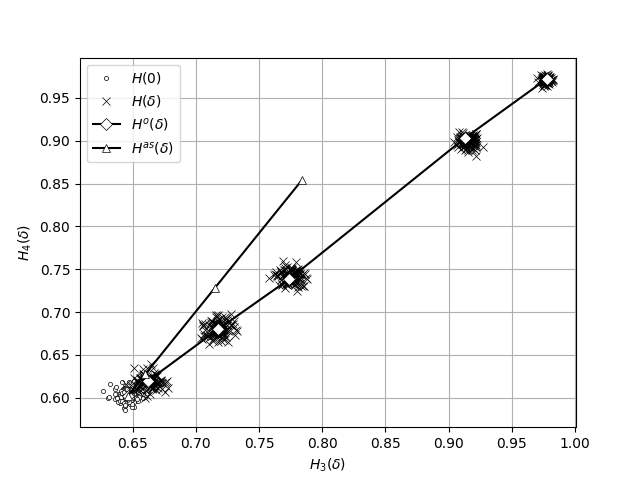
\includegraphics[width=0.5\linewidth]{lda.png}}
		\caption{График зависимости энтропии $H_4{(\delta)}$ от $H_3{(\delta)}$ при различных долях вкраплений}
		\label{ris:"lda.png"}
	\end{figure}
	\newpage
\subsection{Вывод}
Методом линейного дискриминантного анализа на основании энтропийных характеристик $(H_3(\delta), H_4(\delta))$ можно определить наличие вкраплений в последовательность с вероятностью ошибки второго рода 5\% при доле вкраплений $\delta \geq 0.1$.





\clearpage
\newpage
\section{Исследование реальных данных на основании изображений в формате JPEG}
Формат файла JPEG (Joint Photographic Experts Group - Объединенная экспертная группа по фотографии, произносится "джейпег) был разработан компанией C-Cube Microsystems как эффективный метод хранения изображений с большой глубиной цвета, например, получаемых при сканировании фотографий с многочисленными едва уловимыми (а иногда и неуловимыми) оттенками цвета. Самое большое отличие формата JPEG от других рассмотренных здесь форматов состоит в том, что в JPEG используется алгоритм сжатия с потерями (а не алгоритм без потерь) информации. Алгоритм сжатия без потерь так сохраняет информацию об изображении, что распакованное изображение в точности соответствует оригиналу. При сжатии с потерями приносится в жертву часть информации об изображении, чтобы достичь большего коэффициента сжатия. Распакованное изображение JPEG редко соответствует оригиналу абсолютно точно, но очень часто эти различия столь незначительны, что их едва можно (если вообще можно) обнаружить.

Процесс сжатия изображения JPEG достаточно сложен и часто для достижения приемлемой производительности требует специальной аппаратуры. Вначале изображение разбивается на квадратные блоки со стороной размером 8 пиксел. Затем производится сжатие каждого блока отдельно за три шага. На первом шаге с помощью формулы дискретного косинусоидального преобразования (DCT) производится преобразование блока 8х8 с информацией о пикселах в матрицу 8x8 амплитудных значений, отражающих различные частоты (скорости изменения цвета) в изображении. На втором шаге значения матрицы амплитуд делятся на значения матрицы квантования, которая смещена так, чтобы отфильтровать амплитуды, незначительно влияющие на общий вид изображения. На третьем и последнем шаге квантованная матрица амплитуд сжимается с использованием алгоритма сжатия без потерь.

Поскольку в квантованной матрице отсутствует значительная доля высокочастотной информации, имеющейся в исходной матрице, первая часто сжимается до половины своего первоначального размера или даже еще больше. Реальные фотографические изображения часто совсем невозможно сжать с помощью методов сжатия без потерь, поэтому 50\%-ное сжатие следует признать достаточно хорошим. С другой стороны, применяя методы сжатия без потерь, можно сжимать некоторые изображения на 90\%. Такие изображения плохо подходят для сжатия методом JPEG.

При сжатии методом JPEG потери информации происходят на втором шаге процесса. Чем больше значения в матрице квантования, тем больше отбрасывается информации из изображения и тем более плотно сжимается изображение. Компромисс состоит в том, что более высокие значения квантования приводят к худшему качеству изображения. При формировании изображения JPEG пользователь устанавливает показатель качества, величине которого "управляет" значениями матрицы квантования. Оптимальные показатели качества, обеспечивающие лучший баланс между коэффициентом сжатия и качеством изображения, различны для разных изображений и обычно могут быть найдены только методом проб и ошибок.

В качестве контейнера рассматривалась последовательность младших бит ДКП коэффициентов jpeg изображения.\\
Пусть $X={x_1,..., x_n}$ последовательность младших бит коэффициентов ДКП изображения.
\begin{equation}
\hat{p}\{x=1\}=\frac{\sum^n_{i=1}x_i}{n}
\end{equation}
На основании экспериментального исследования некоторой базы изображений и формате jpeg можно сделать вывод, что экпериментальная оценка вероятности появления единичного бита находится в интервале  [0.350705572829466, 0.480247228960331] для исследуемой базы изображений. Следовательно младшие биты ДКП коэффициентов изображений формата jpeg не являются равномерно распределенными. Поэтому изображения в формате jpeg не являются подходящим контейнером для исследования изложеной теории обнаружения вкраплений. \\
\begin{figure}[h]
	\center{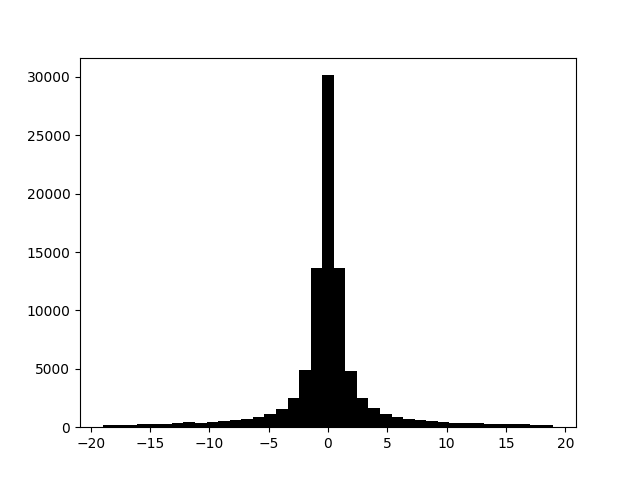
\includegraphics[width=0.5\linewidth]{hist1.png}}
	\caption{Гистограмма ДКП коэффициентов jpeg изображения}
	\label{ris:"hist1.png"}
\end{figure}
\clearpage
\newpage
\section{Компьютерные эксперименты}
 
\vspace*{1cm}
	\begin{figure}[h]
		\center{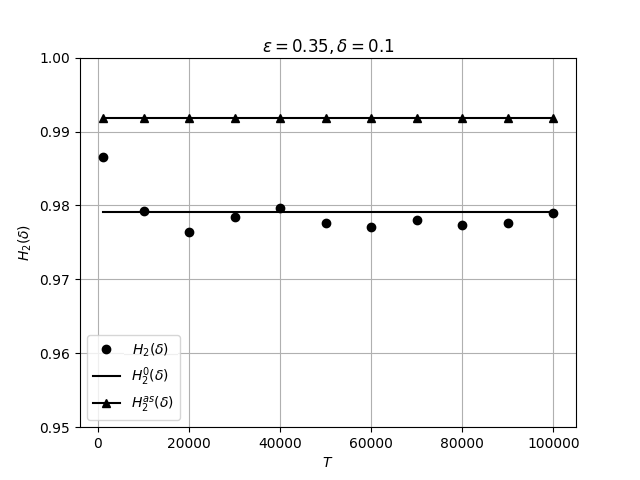
\includegraphics[width=0.6\linewidth]{h2_01.png}}
		\caption{График зависимости энтропии $H_2{(\delta)}$ от длины последовательности при  $\delta = 0.1$}
		\label{ris:"h2_01.png"}
	\end{figure}
	\begin{figure}[h]
		\center{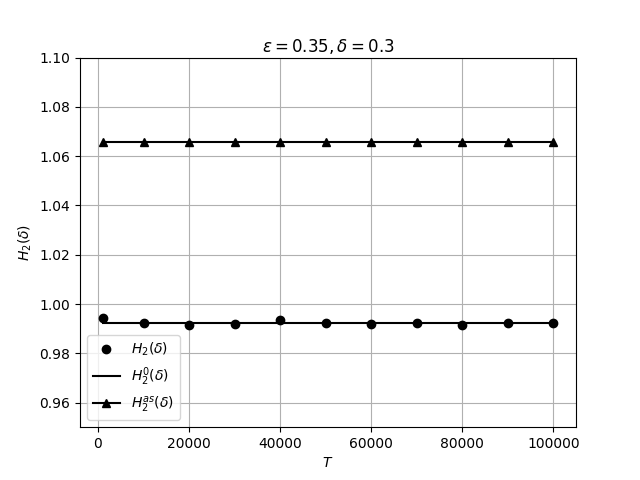
\includegraphics[width=0.6\linewidth]{h2_03.png}}
		\caption{График зависимости энтропии $H_2{(\delta)}$ от длины последовательности при  $\delta = 0.3$}
		\label{ris:"h2_03.png"}
	\end{figure}
		\begin{figure}[h]
			\center{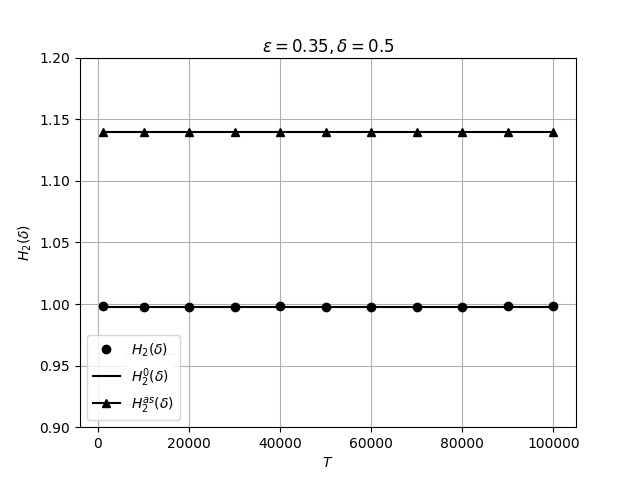
\includegraphics[width=0.8\linewidth]{h2_05.png}}
			\caption{График зависимости энтропии $H_2{(\delta)}$ от длины последовательности при  $\delta = 0.5$}
			\label{ris:"h2_05.png"}
		\end{figure}
			\begin{figure}[h]
				\center{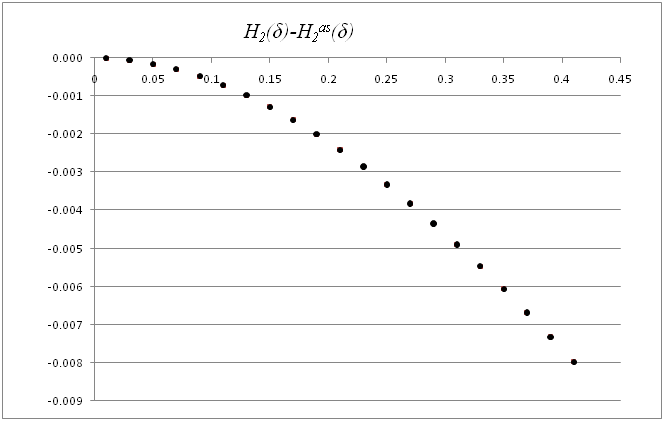
\includegraphics[width=0.8\linewidth]{h2.png}}
				\caption{График зависимости разности ассимптотического и точного значений энтропии биграммы от доли вкрапления}
				\label{ris:"h2.png"}
			\end{figure}
		
	\begin{figure}[h]
		\center{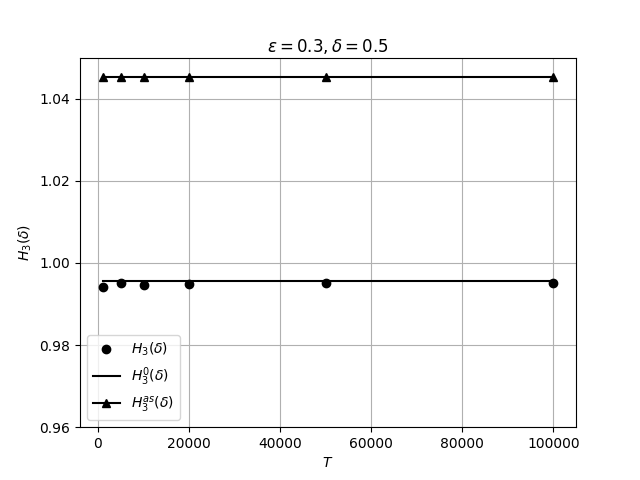
\includegraphics[width=0.8\linewidth]{h3_05.png}}
		\caption{График зависимости энтропии $H_3{(\delta)}$ от длины последовательности при  $\delta = 0.5$}
		\label{ris:"h3_05.png"}
	\end{figure}
	\begin{figure}[h]
		\center{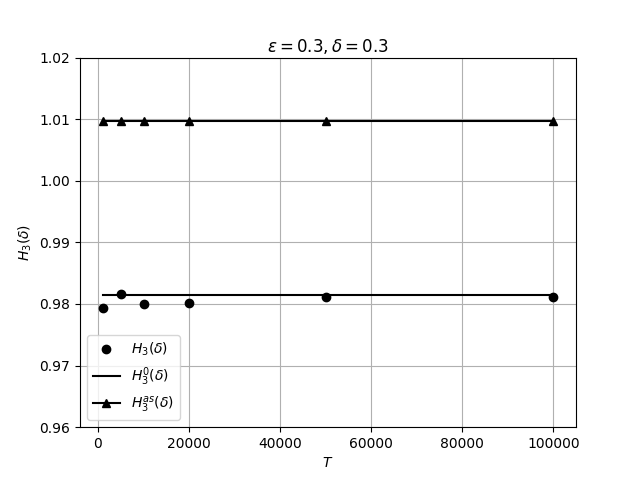
\includegraphics[width=0.8\linewidth]{h3_03.png}}
		\caption{График зависимости энтропии $H_3{(\delta)}$ от длины последовательности при  $\delta = 0.3$}
		\label{ris:"h3_03.png"}
	\end{figure}
		\begin{figure}[h]
			\center{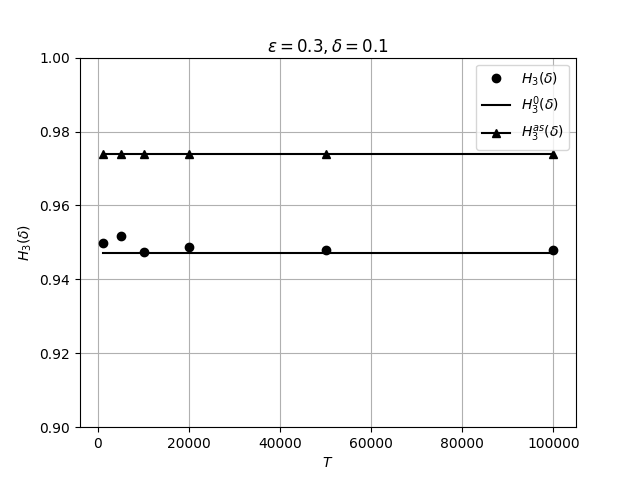
\includegraphics[width=0.8\linewidth]{h3_01.png}}
			\caption{График зависимости энтропии $H_3{(\delta)}$ от длины последовательности при  $\delta = 0.1$}
			\label{ris:"h3_01.png"}
		\end{figure}
			\begin{figure}[h]
				\center{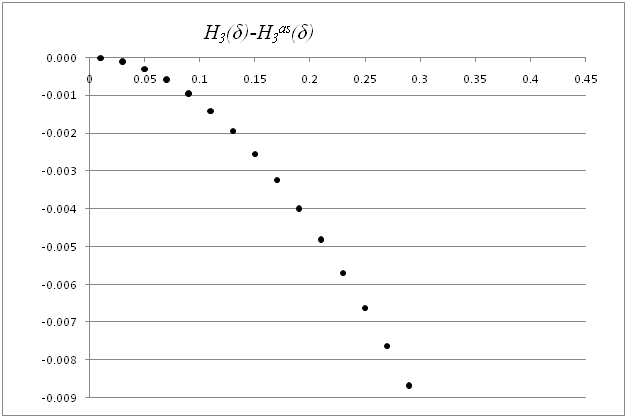
\includegraphics[width=0.8\linewidth]{h3.png}}
				\caption{График зависимости разности ассимптотического и точного значений энтропии 3-граммы от доли вкрапления}
				\label{ris:"h3.png"}
			\end{figure}
			\begin{figure}[h]
				\center{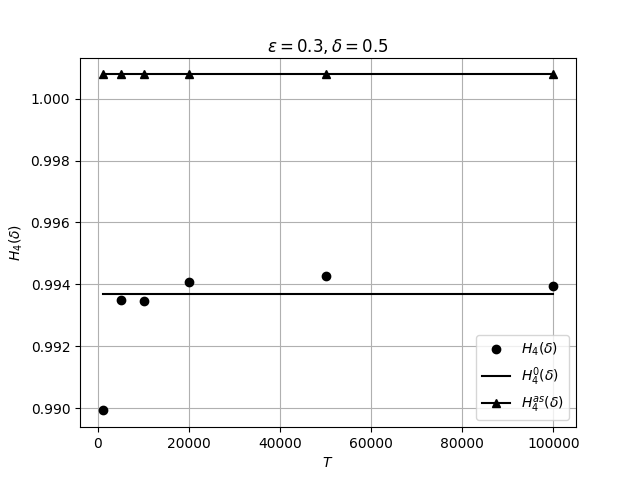
\includegraphics[width=0.8\linewidth]{h4_05.png}}
				\caption{График зависимости энтропии $H_4{(\delta)}$ от длины последовательности при  $\delta = 0.5$}
				\label{ris:"h4_05.png"}
			\end{figure}
				\begin{figure}[h]
					\center{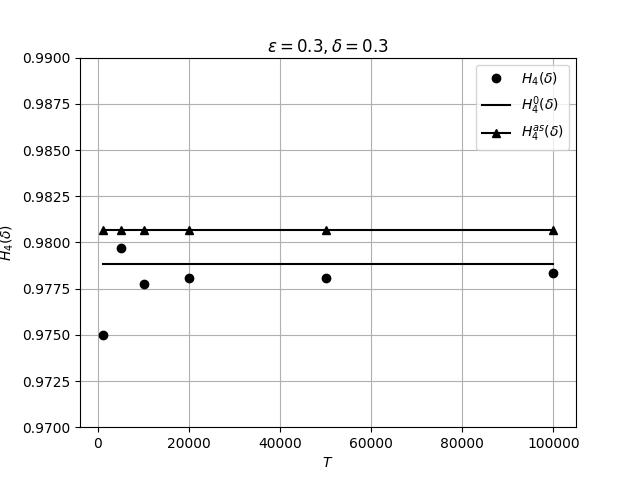
\includegraphics[width=0.8\linewidth]{h4_03.png}}
					\caption{График зависимости энтропии $H_4{(\delta)}$ от длины последовательности при  $\delta = 0.3$}
					\label{ris:"h4_03.png"}
				\end{figure}
					\begin{figure}[h]
						\center{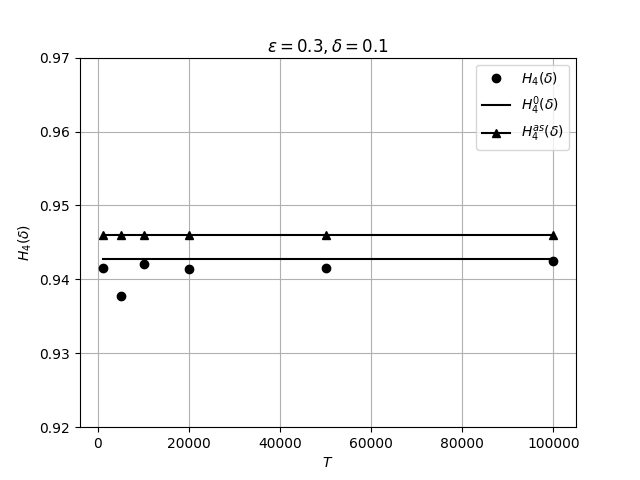
\includegraphics[width=0.8\linewidth]{h4_01.png}}
						\caption{График зависимости энтропии $H_4{(\delta)}$ от длины последовательности при  $\delta = 0.1$}
						\label{ris:"h4_01.png"}
					\end{figure}
						\begin{figure}[h]
							\center{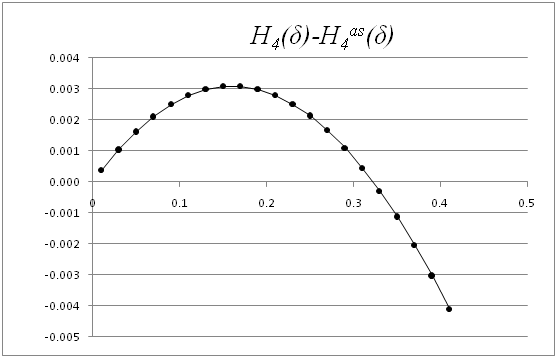
\includegraphics[width=0.8\linewidth]{h4.png}}
							\caption{График зависимости разности ассимптотического и точного значений энтропии биграммы от доли вкрапления}
							\label{ris:"h4.png"}
						\end{figure}
					
							\begin{figure}[h]
								\center{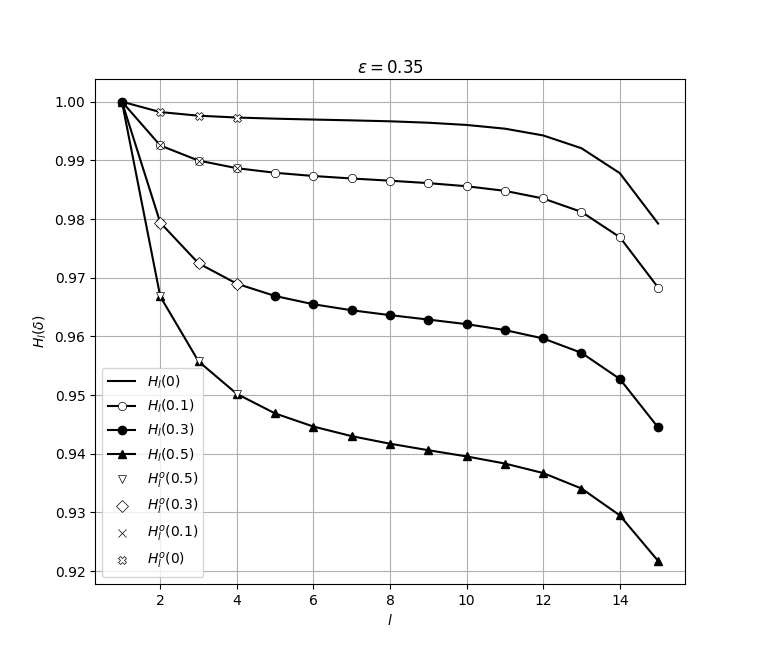
\includegraphics[width=1\linewidth]{h_l.png}}
								\caption{Семейство графиков зависимости энтропии $H_l{(\delta)}$ от L при различных $\delta$}
								\label{ris:"h_l.png"}
							\end{figure}
						
						
						
					


\clearpage




\begin{thebibliography}{0}
	\bibitem{duhin}
	А. А. Духин: Теория информации - М.: "Гелиос АРВ", 2007.
	\bibitem{agranovskiy} 
	А.В. Аграновский, А. В. Балакин: Стеганография, цифровые водяные знаки о стегоанализ - М.: Вузовская книга, 2009.
	\bibitem{gribunin}
	 В. Г. Грибунин, И. Н. Оков, И. В. Туринцев: Цифровая стеганография - М.: Солон-Прессб, 2002.
	\bibitem{varnoskiy}
	Н. П. Варновский, Е. А. Голубев, О. А. Логачев: Современные направления стеганографии. Математика и безопасность информационных технологий. Материалы конференции в МГУ 28-29 октября 2004 г., МЦМНО, М., 2005, с. 32-64.
	\bibitem{harin}
	Ю. С. Харин [и др.]: Криптология - Минск: БГУ, 2013.
	\bibitem{vecherko}
	Ю. С. Харин, Е. В. Вечерко "Статистическое оценивание параметров модели вкраплений в двоичную цепь Маркова", Дискрет. матем., 25:2 (2013), 135-148.
\end{thebibliography}

\end{document}
